%% This is an example first chapter.  You should put chapter/appendix that you
%% write into a separate file, and add a line \include{yourfilename} to
%% main.tex, where `yourfilename.tex' is the name of the chapter/appendix file.
%% You can process specific files by typing their names in at the 
%% \files=
%% prompt when you run the file main.tex through LaTeX.
\chapter{Implementation}\label{intro-ch}

\section{Spark}

All of the code was being implemented in Spark. As mentioned before, Spark is the next 
generation of map reduce and has received a huge amount of support. Although the code was implemented in Spark, 
it could also be implemented in map reduce to achieve similar gains. Matei Zaharia added code 
that allowed the tracking of sizes of map output files.   

\section{ShuffledRDD}

As mentioned before, the RDD is the main interface to interact with data in Spark.
The RDD we developed we developed basically is a new version of ShuffledRDD. Our version
of ShuffledRDD2 is basically a new version of the RDD. It takes in a shuffle dependency
, which is basically a bunch of partitions that have finished the map output stage. As mentioned before,
in a general ShuffledRDD just does basic logic, and does not do balancing. Our dependency
basically takes in a number of reducers and then best tries to balance the partitions of the reducer.
As this is more a proof of concept, our version of ShuffledRowRDD will only output consecutive partitions to one
reducer. In other words, it is impossible for a reducer to have partitions 1 and 3, without having partition 2. 
In the future, we hope to expand the RDD so that it best balances the parttions.

\section{Joins}

\subsection{ShuffleReader Changes}

We added some flexibility to how shuffles are fetched. As mentioned in the shuffle section,
we would like the bigger RDD to stay in place. The current interface allows a reducer to pick a specific partition
from the mapper and autofetched it from all of the mappers. In other words, you could only request partition 1 from
all the mappers. This would be extremely problematic for the broadcast join as we want none of the bigger RDD to move
at all. The key part of the RDD interface is basically how a new reducer partition is computed from the old map partition.
Thus, each of the reducer partitions ic computed by requesting the necessary amount of partitions from the mappers as described above.   

\subsection{ShuffleJoinRDD and BroadcastJoin RDD}

We implement two different type of RDD's, the ShuffleJoinRDD and the
BroadcastJoinRDD. Both of these RDD's take two shuffle dependencies, which remember
are basically the outputs of map stages, partitioned in a certain way. These 
dependencies must be partitioned in the same way. Otherwise, we have no way
of ensuring that the two keys are in the same partition.  
\\

The ShuffleJoinRDD is implemented in a manner similar to the way to a regular shuffledRDD is  
The shuffledependency basically fetches a number of partitions of the shuffle dependency. 
It ensures that the partitions that it fetches are the same, i.e. reducer partition 1 will fetch dataset 1 partition 1 and dataset2
partition 1 from all of the workers. Once these partitions are fetched, we basically form a map with the smaller partition present
and iterate through the bigger partition, seeing if there are keys present in this map. If so, we add this to ourput.\\
The BroadcastJoinRDD implements the broadcast shuffle that was explained above.
For each reduce partition, it requests one local partition from the mapper from the bigRDD. To be clear,
we use the new api and are just requesting one partition of the bigRDD from one mapper. We then request 
all of the paritions from the smaller RDD, thus giving us all of the smaller RDD. We then use the same strategy
to actually join them as the shuffle join rdd.

\subsection{Joins in Spark SQL}

Although the RDD interface can be used, many programmers and data analysts prefer not to use this interface
and are more familiar with the spark interface. Thus, Spark offers a sql like interface. Within, this interface
they offer a join operator and functions just like a join that was explained above. Although this code is written in a sql like statement,
the code is still converted and executed by using RDD's.\\

Because we are not just using the RDD interface, the exact way we implement our code changes is a 
little more compliacted. We only implement our code is a specific technique for sort merge join.
One key change change is that we add a flag indicating whether our join is a sort merge join. Because the query planner determines the type of join, we only implement our join type
for sort merge join.\\

Although the exact semantics for how a sort merge join can be found here,
the sort merge join like the shuffle requires everyting that needs to be compared together to be on the machine.
The main difference is that when it finds intersections, instead of putting one of the datasets in a map like interface,
it sorts both partitions, and then iterates through them and advances the partitions. \\

The following example in Figure~\ref{fig:exchange} details the inner workings
of how the query plan works. The first part of the plan is called the exchanges. 
The exchanges are where pretty much all of my changes happened. We create ShuffledRowRDds which
are pretty much equivalent to regular shuffle RDD's, but are slightly different as they represent
rows as we are dealing with tables in this spark sql configuration. The program will 
compare partition 1 of our ShuffledRowRDD to partition 1 of the other ShuffledRowRDD. Therefore,
we need to ensure that they match up accordingly. This is very similar to the key concepts between the
broadcast join and shuffled RDD.Within the shuffledRowRDD,
we look at the total size of the partitions of each dataset. If one is smaller then a particular
threshold and the other is not, then we do a a broadcast join,
Both the threshold and the ability to do the sort merge join are set through a flag that can be
triggered in the conf field.\\

In the broadcast join, the shuffledRowRDD for the big RDD  produced is basically
the same as the initial RDD. However, for the smaller shuffledRowRDD, each partition contains
all of the partitions from the data. We set the number of partitions it has to be equal to the number of partitions
the smaller one has. The shuffle join is what happens by default without our code being implemented. It sets,
the number of partitions for each ShuffledRowRDD to be some number that is set in the conf. It then ensures that partition 1 of 
the ShuffleRowRDD, i.e. will have the coressponding partition for partition one in shuffledRowRDD 1 and shuffledRowRDD 2. 

The rest of the query plan is basically used for the sort merge join.
The sort feature sorts the RDd. The ZippedPartions part is used as we iterate through the two sorted
lists for merging them.
 
\begin{figure}[h]
\begin{center}
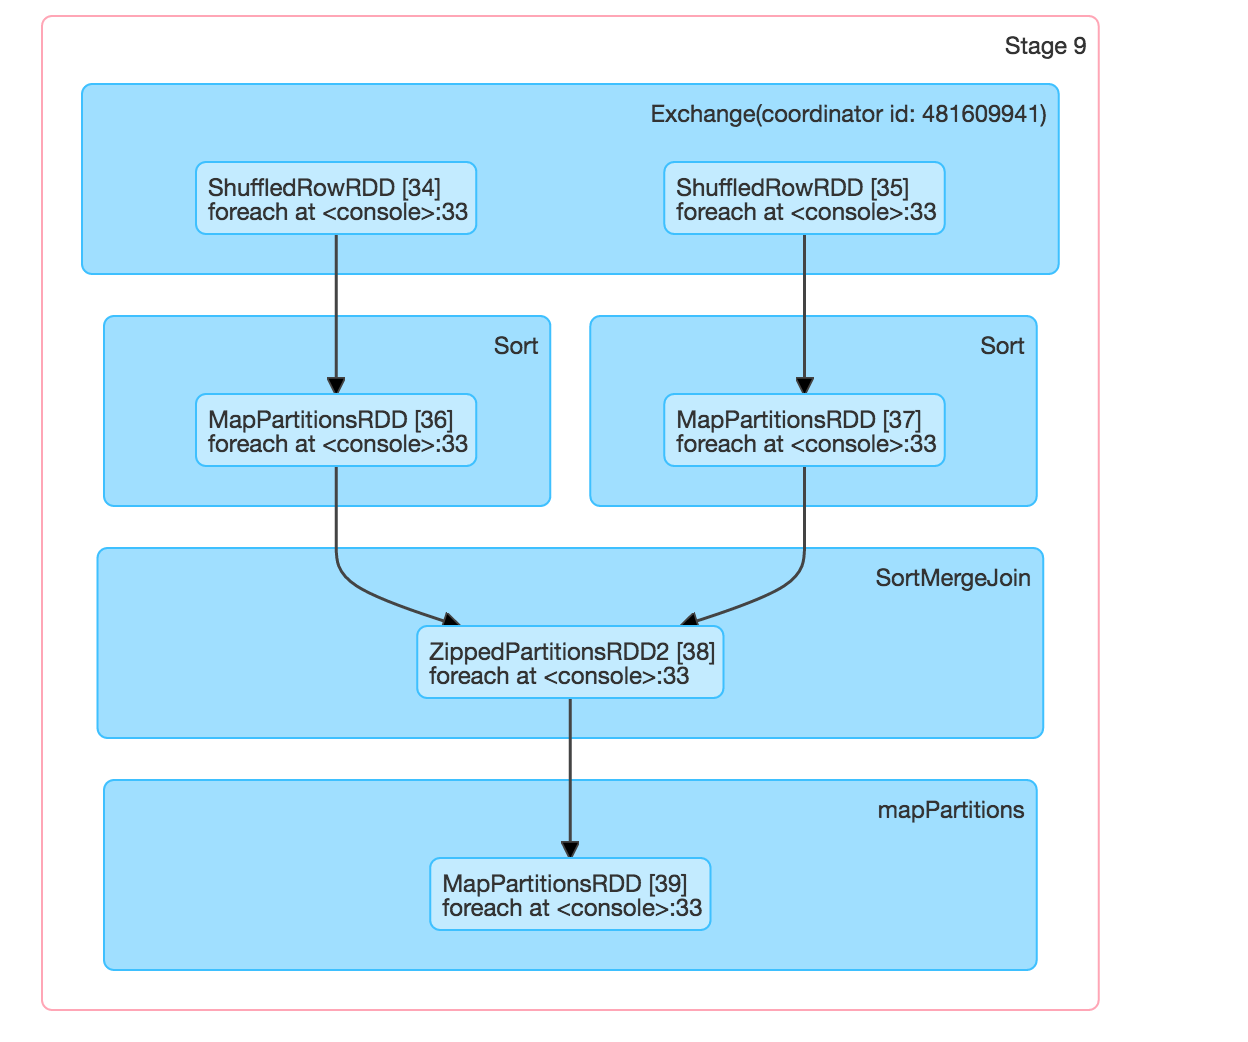
\includegraphics[scale=1.0]{./img/exchange.png}
\caption{Plan for Sort Merge Join}
\label{fig:exchange}
\end{center}
\end{figure}


